To fully understand how residential consumers adjust their electricity consumption behavior as a set of reactions to the price changes in and near the peak rate period under the TOU price structures, it is necessary to examine the relationship between the size of price increases in the period and the electricity savings from each of the two distinct sources for different points in time where electricity is consumed. For that reason, I quantitatively determine the relationship by utilizing the following econometric model:
\begin{equation}
\small
\begin{split}
    kWh_{ith} \ 
    & = \ \beta_{1} HDD_{t} \ + \ \beta_{2} HDD_{t}^{*} \\
    & \hspace{0.7cm} + \ \beta_{3} \mathds{1}[\text{Treatment}]_{i} \ + \ \beta_{4} \mathds{1}[\text{Treatment}]_{i} \Delta RC_{i} \\
    & \hspace{0.7cm} + \ \beta_{5} HDD_{t} \mathds{1}[\text{Treatment}]_{i} \ + \ \beta_{6} HDD_{t} \mathds{1}[\text{Treatment}]_{i} \Delta RC_{i} \\
    & \hspace{0.7cm} + \ \beta_{7} HDD_{t}^{*} \mathds{1}[\text{Treatment}]_{i} \ + \ \beta_{8} HDD_{t}^{*} \mathds{1}[\text{Treatment}]_{i} \Delta RC_{i} \\
    & \hspace{0.7cm} + \ \beta_{9} \mathds{1}[\text{Post}]_{t} \ + \ \beta_{10} HDD_{t} \mathds{1}[\text{Post}]_{t} \ + \ \beta_{11} HDD_{t}^{*} \mathds{1}[\text{Post}]_{t} \\
    & \hspace{0.7cm} + \ \beta_{12} \mathds{1}[\text{Treatment \& Post}]_{it} \ + \ \beta_{13} \mathds{1}[\text{Treatment \& Post}]_{i} \Delta RC_{i} \\
    & \hspace{0.7cm} + \ \beta_{14} HDD_{t} \mathds{1}[\text{Treatment \& Post}]_{it} \ + \ \beta_{15} HDD_{t} \mathds{1}[\text{Treatment \& Post}]_{i} \Delta RC_{i} \\
    & \hspace{0.7cm} + \ \beta_{16} HDD_{t}^{*} \mathds{1}[\text{Treatment \& Post}]_{it} \ + \ \beta_{17} HDD_{t}^{*} \mathds{1}[\text{Treatment \& Post}]_{i} \Delta RC_{i} \ + \ \alpha_{dw} \ + \ \epsilon_{ith}
\end{split}
\end{equation}
The model is the same with (XYZ) except for interaction terms between treatment-status-relevant indicator variables (i.e., $\mathds{1}[\text{Treatment}]_{i}$ and $\mathds{1}[\text{Treatment \& Post}]_{it}$) and $\Delta RC_{i}$, where $\Delta RC_{i}$ is the difference between the peak-hour prices in the treatment period and the flat rate in the baseline period. The coefficients of those interaction terms capture the impacts of deploying the TOU tariffs on household electricity consumption as a linear function of the amount of peak-demand-hour price changes.

\begin{table}
    \caption{Treatment Effects as a Linear Function of the Price Changes in the Peak Rate Period}
\end{table}

\begin{figure}[!th]
\centering
%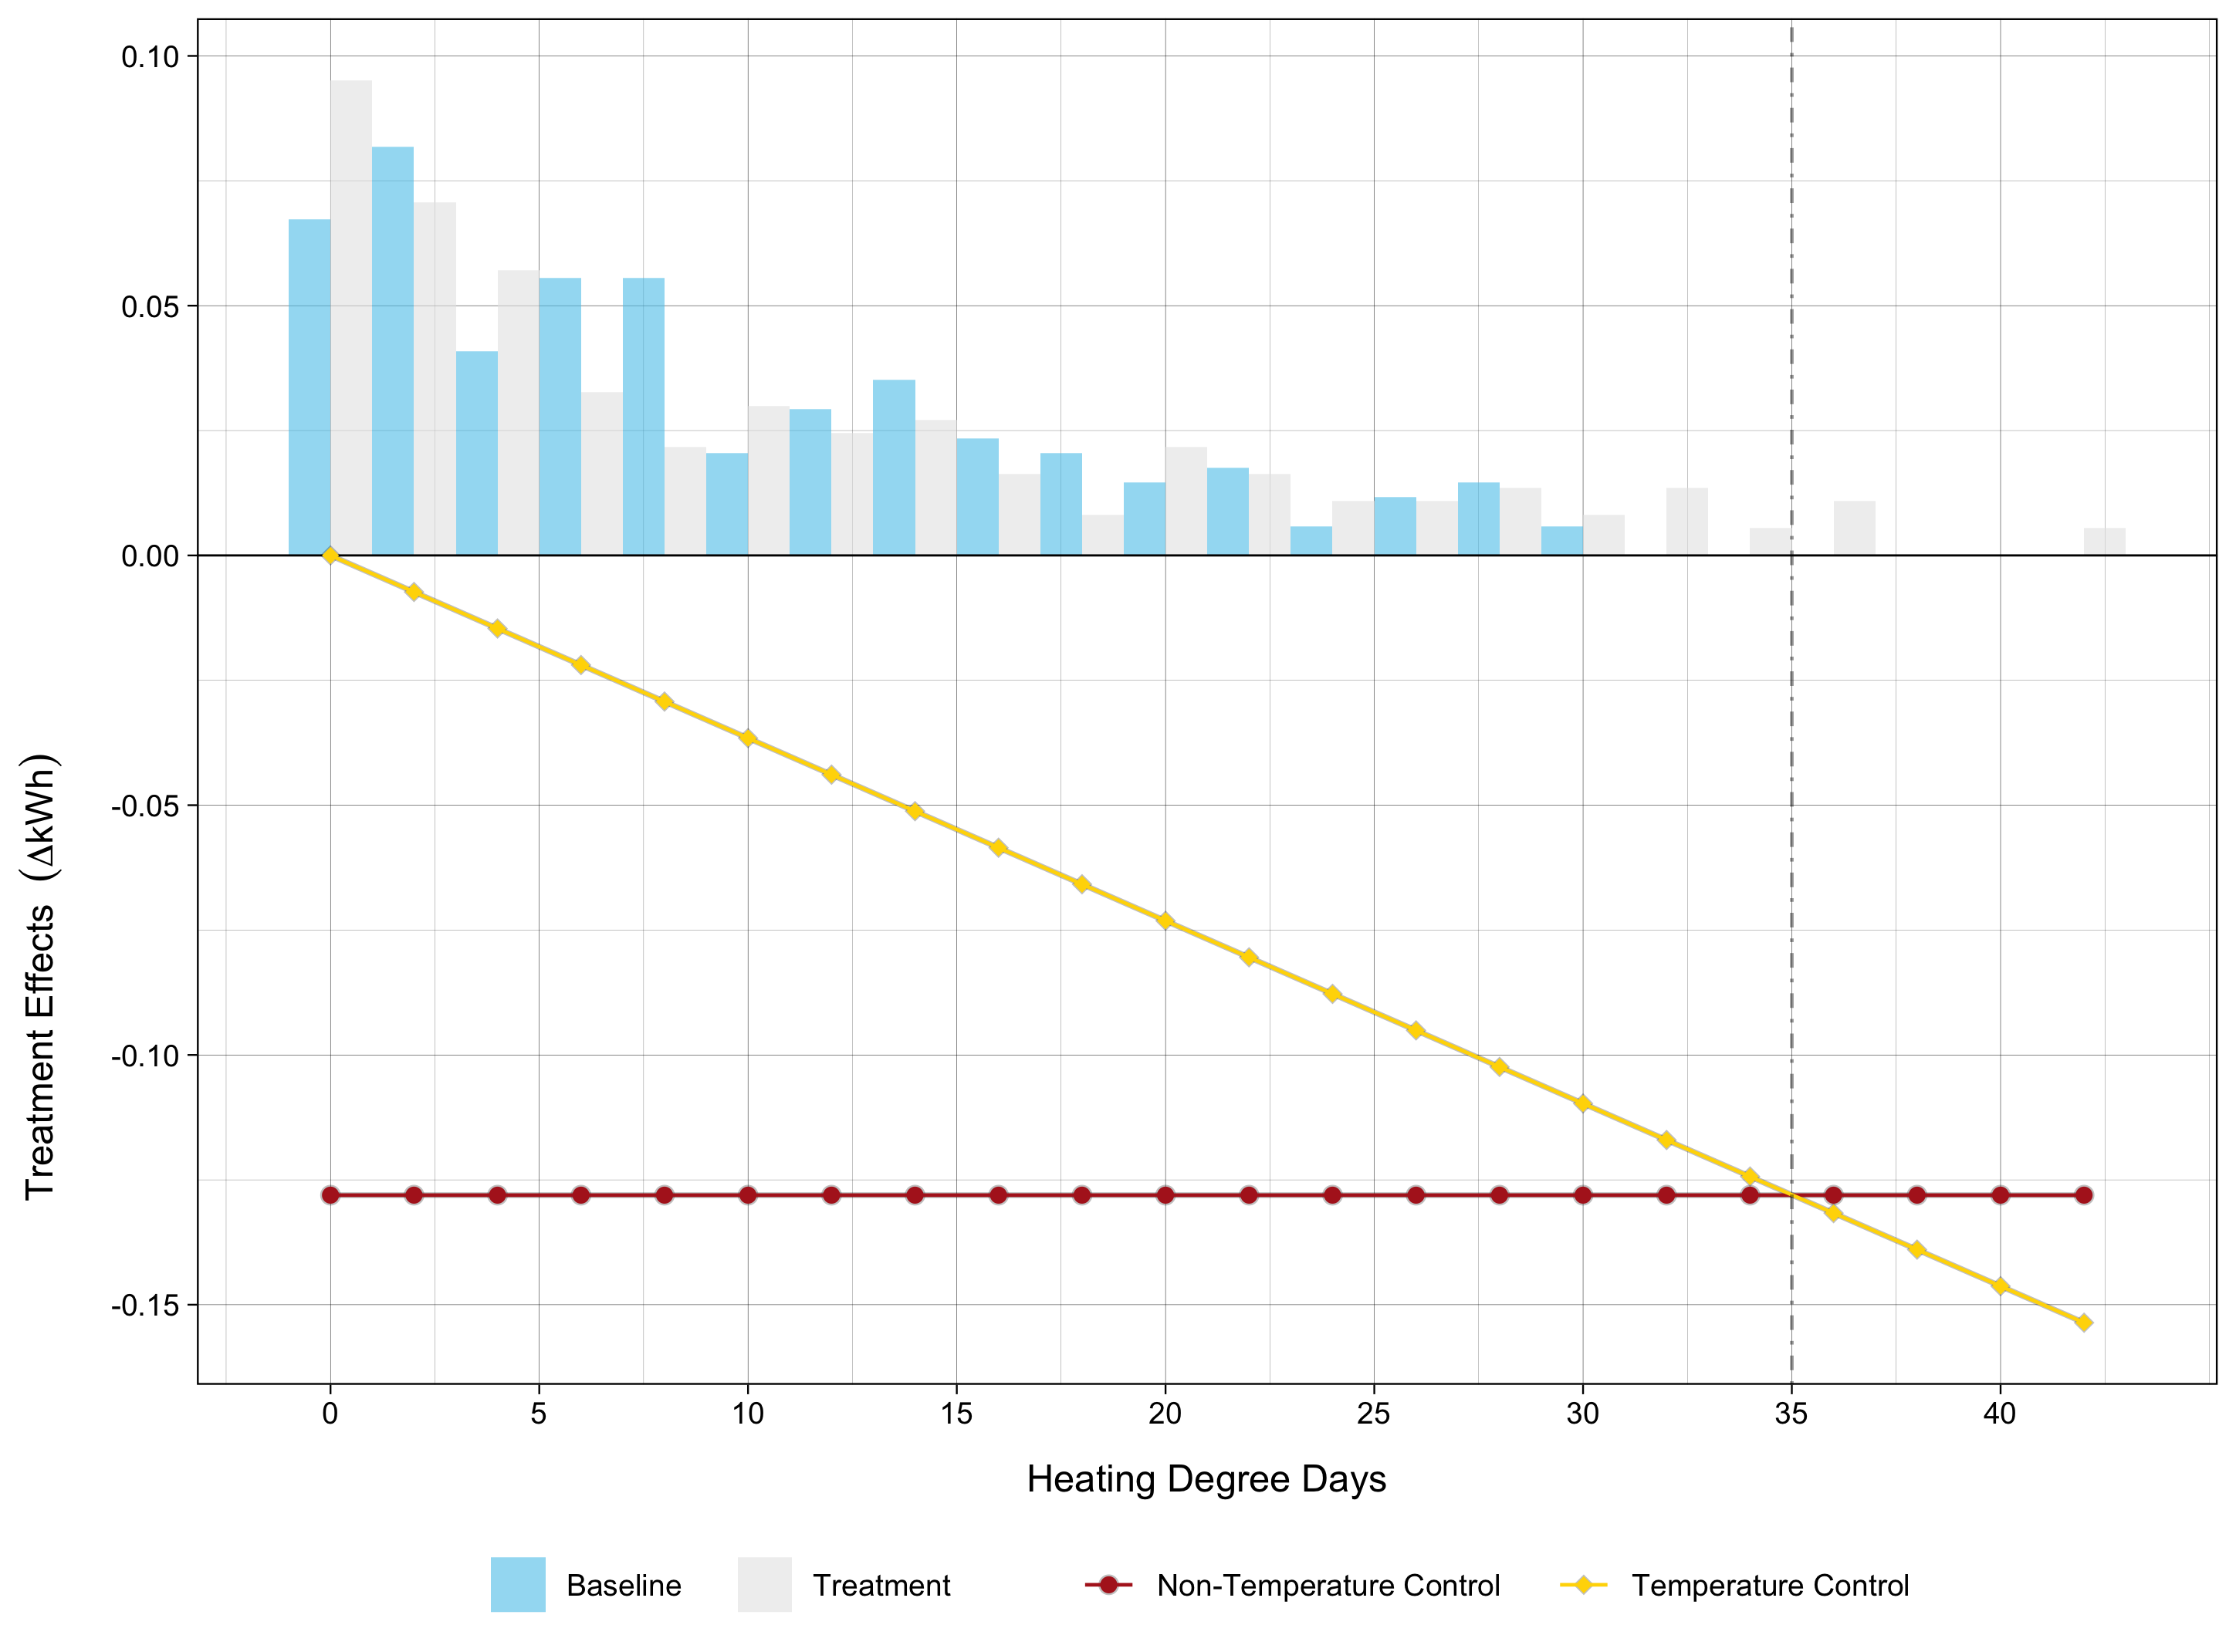
\includegraphics[scale = 0.16]{03_Chapter-2/00A_Figures/Figure_Breakdown-of-Hourly-ATEs-in-the-Peak-Rate-Period.png}
\caption{Treatment Effects as a Linear Function of the Price Changes in the Peak Rate Period}
\label{Figure:Treatment-Effects-as-a-Linear-Function-of-the-Price-Changes-in-the-Peak-Rate-Period}
\end{figure}

The estimates of the six coefficients of interest (i.e., from $\beta_{12}$ to $\beta_{17}$) presented in Table XYZ are summarized graphically in Figure XYZ. And this figure, showing estimated treatment effects and predicted electricity savings for each of the three intervals, re-confirms the finding of price insensitivity in \cite{Peaking-Interest:How-Awareness-Drives-the-Effectiveness-of-Time-of-Use-Electricity-Pricing_Prest_2020}. In the peak rate period, the non-for-heating-associated electricity savings were directly proportional to the rate changes in the period. On the contrary, at a given daily HDDs, the for-heating-related electricity savings, having HDD-varying U-shaped profile, were inversely proportional to the magnitude of peak-demand-hour tariff changes. As shown in the figure clearly, the differences in the predicted electricity savings over the degree of price changes are apparent when the savings stemming from the two distinct sources are examined individually. The differences, however, are seemingly dampened when the electricity savings are aggregated due to the opposite correlations. Indeed, this empirical result is consistent with the finding discussed in the previous work that households were unusually insensitive to the size of the price changes in the peak rate period. 

The opposite order in estimated treatment effects between the two sources of electricity savings also holds in the two-hour-length pre-peak interval, although in a contrary manner. The interval shows directly proportional savings from electricity consumption for temperature-control uses to changes in the peak rate. By contrast, the variations in non-temperature-control-related electricity consumption caused by TOU prices exhibit an inverse relationship with the price changes in the peak rate period. For the same reason, the aggregated treatment effects of the TOU tariffs are seemingly less sensitive to prices. Note that regarding the electricity consumption for heating, the TOU tariffs played a role only when temperatures were sufficiently low. 

Residential consumers adjust their electricity consumption behavior during the two-hour-length post-peak period as well. As in the pre-peak interval, the savings stemming from non-for-heating-associated electricity consumption were inversely proportional to the price jumps in the peak rate period. In the case of electricity consumption for heating, the TOU program provoked additional consumption in that interval, especially on freezing days. The amount of the added for-heating-relevant household electricity consumption increased as the price variations in the peak-hour interval diminished. Therefore, the resulting treatment effects (i.e., the aggregated treatment effects) also agree with the finding of price insensitivity in the previous paper. 

In summary, under TOU pricing, the level of price changes, not merely its existence, still matters to residential consumers. The empirical results above suggest that the opposite order in estimated treatment effects between non-temperature- and temperature-control uses of electricity makes Irish households appear to violate the law of demand. In other words, due to the opposite order, their high sensitivity to the TOU prices is revealed only when household electricity consumption is disaggregated to the two distinct sources of electricity savings. Together with the empirical findings in previous sections, the results imply that three simultaneously interacting factors govern the dynamics of residential electricity consumption under TOU pricing: the timing when electricity is consumed, daily HDDs, and the magnitude of price increases in the peak rate period. 

